\chapter{Grundlagen}
\label{cha:grundlagen}

% Abschnitt: Quartettspiel
\section{Quartettspiel}
\label{sec:grundlagen:quartettspiel}

Zum Quartettspielen sind natürlich einige Regeln notwendig, die im Folgenden erklärt werden. \\
Gespielt wird Eins gegen Eins, Spieler gegen Computer. Zuerst wählt der Spieler den Schwierigkeitsgrad (leicht, mittel oder schwer) des Computers, dann den Spielmodus und das Limit für das Spielende (Zeit-, Runden- oder Punktemodus und entsprechend die Spielzeit, Runden- oder Punkteanzahl). Danach wird ein Deck gewählt und gemischt. Computer und Spieler bekommen jeweils die Hälfte der Karten verdeckt auf einem Stapel, bei dem immer nur die oberste Karte sichtbar ist, und es wird zufällig bestimmt wer mit dem ersten Zug beginnen darf. Ein Zug läuft im Grunde genauso ab wie beim ``echten'' Quartett: Der Spieler, der am Zug ist, wählt ein Attribut (Beispiel in einem Autoquartett: Höchstgeschwindigkeit) und nennt den entsprechenden Wert. Der andere Spieler gibt nun ebenfalls seinen Wert bei dem gewählten Attribut bekannt (Beispiel von oben: Höchstgeschwindigkeit) und die Werte werden verglichen. Für jedes Attribut wurde vor dem Spiel festgelegt ob für dieses ein höherer oder niedrigerer Wert gewinnt. Darauf basierend wird nun der Vergleich durchgeführt. Der Spieler mit dem besseren Wert gewinnt den Vergleich, bekommt beide Karten unter seinen Stapel und darf im nächsten Vergleich das Attribut wählen. Bei einem Unentschieden behält jeder seine Karte, legt sie unter seinen Stapel und der Spieler, der das Attribut gewählt hat, wählt auch das nächste. Das Spiel ist zu Ende, wenn ein Spieler keine Karten mehr auf seinem Stapel hat, oder wenn das Limit des gewählten Spielmodus erreicht ist (Zeit abgelaufen / alle Runden ausgespielt / Punktelimit erreicht).

Dies sind die normalen Regeln und Spielmodi für ein Quartettspiel. In unserer App gibt es aber zusätzlich neben dem normalen Modus (bei dem jeweils, wie festgelegt, der höhere oder niedrigere Wert den Vergleich gewinnt) auch noch den sog. ``Insane-Modus'', bei dem jeweils nicht der vorher festgelegte höhere oder niedrigere Wert gewinnt, sondern genau umgekehrt. Damit es im Spiel dennoch nicht zu Verwirrungen kommt, ist neben jedem Attribut ein Pfeil, der angibt, ob (im aktuellen Modus) ein höherer oder niedrigerer Wert beim Vergleich gewinnt.
Unabhängig vom Insane-Modus kann der Benutzer zusätzlich entscheiden, ob er den Expertenmodus spielen möchte oder nicht. Der Expertenmodus ist jedoch nichts für Anfänger, denn es werden die Werte einer Karte ``zensiert'' (durch ein '?' ersetzt), sodass man das Deck bzw. die Karten schon ein bisschen besser kennen muss, um hier erfolgreich zu sein.


% Abschnitt: Mobile Plattform
\section{Mobile Plattform}
\label{sec:grundlagen:plattforml}

Android ist ein mobiles Betriebssystem, also für Smartphones und Tablets, das von Google entwickelt wurde und auf Linux basiert. Die App-Entwicklung ist geprägt durch einzelne Aktivitäten (eine Aktivität ist eine einzelne Bildschirmseite einer Android-App), die miteinander kommunizieren und in ihrer 'Lebenszeit' ein vorgegebenes Zustandsmodell \ref{figure:androidZustandsmodell} durchlaufen.

\begin{figure}[htp]
	\centering
  	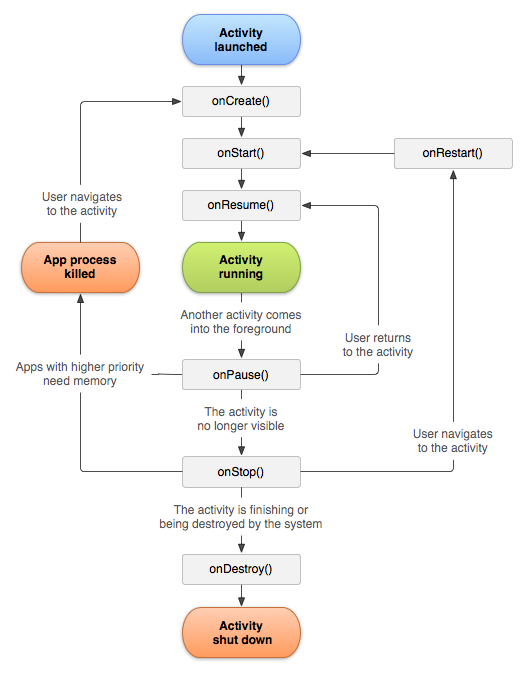
\includegraphics[width=0.33\textwidth]{img/modelle/AndroidZustandsmodell.png}
	\caption[Android Zustandsmodell]{Android Zustandsmodell\protect\footnotemark}
	\label{figure:androidZustandsmodell}
\end{figure}
\footnotetext{http://www.javatpoint.com/images/androidimages/Android-Activity-Lifecycle.png}

Dieses Zustandsmodell ist auch anfangs einer der Nachteile von Android, da es nicht so leicht zu verstehen ist und uns einige Probleme bereitet hat. Nachdem wir uns aber im Laufe der App-Entwicklung immer mehr mit Android vertraut gemacht haben, war auch das Modell kein Problem mehr, sondern im Gegenteil sehr angenehm, da es sehr logisch und gut durchdacht ist. Eine weitere Schwierigkeit, die während der Entwicklung auftrat, ist die Vielzahl an verschiedenen Android-Versionen und Geräten. Da wir unsere App für so viele Versionen wie möglichen entwickeln wollten, kamen auch einige Probleme auf. Beispielsweise sind manche Libraries oder Frameworks erst ab einer bestimmten Android-Version verfügbar, und die vielen verschiedenen Geräte haben meist unterschiedliche Displaygrößen und Seitenverhältnisse.\\
Die Vorteile von Android überwiegen aber unserer Meinung nach, vor allem, nachdem man sich damit tiefer beschäftigt und sich eingearbeitet hat. Einer der größten Vorteile ist die sehr gute Dokumentation von Android, wodurch das Einlesen in die Möglichkeiten und Funktionen recht leicht ist. Auch die weltweite Verbreitung und Beliebtheit von Android ist hier ein Vorteil, da es sehr viele Entwickler gibt und so jedes Problem schon einmal aufgetreten ist und daher auch meist schon Lösungen oder Hilfestellungen verfügbar sind.

Außerdem wird Android stetig Weiterentwickelt, weshalb immer mehr möglich ist und der Umgang mit bestimmten Funktionen, wie etwa der Zugriff auf Gerätefunktionen wie Kamera oder Galerie, immer leichter wird. Weitere Vorteile für uns sind die Vertrautheit mit Java und die Einfachheit der eigens von Google bereitgestellten Entwicklungsumgebung, ``Android Studio''.

% Abschnitt: Frameworks
\section{Frameworks}
\label{sec:grundlagen:frameworks}
Frameworks sind Ansammlungen von Funktionen, die wiederverwendet werden können um einen gezielten Bereich der Implementierung zu erleichtern und die Anzahl an neu zu implementierenden Funktionen zu verringern.\\
Wir haben in unserer App drei Frameworks als Hilfen genutzt:
\begin{itemize}
\item Picasso\footnote{http://square.github.io/picasso/}: Erlaubt einen wesentlich einfacheren Umgang hinsichtlich Anzeige, (asynchronem) Laden, und Transformation von Bildern.
\item MPAndroidCharts\footnote{https://github.com/PhilJay/MPAndroidChart}: Ermöglicht die Erstellung von Diagrammen - in unserem Fall Kuchendiagramme zur Visualisierung der Statistiken
\item Floating Action Button / Floating Action Menu\footnote{https://github.com/Clans/FloatingActionButton}: Eine Erweiterung des standardmäßigen Floating Action Buttons in Form eines Menüs, das ein- und ausgeklappt werden kann.
\end{itemize}



















